
\documentclass{abgabe}
\begin{document}

\begin{questions}
    \qformat{\thequestion. \textbf{\thequestiontitle} \hfill}
    \titledquestion{Kohäsion und Kopplung}

    \begin{parts}
        \part Beschreiben Sie in eigenen Worten das Prinzip der Kohäsion und Kopplung in der Implementierung von Software-Projekten.
        \begin{solution}
            Als Reaktion auf einen mittelmäßigen Artikel über die Standarddefinitionen von Kohäsion und Kopplung, fasste ein mittlerweile \href{https://www.reddit.com/r/programming/comments/3jeoyh/comment/cup1max/?utm_source=reddit&utm_medium=web2x&context=3}{gelöschter Reddit-User} die beiden Begriffe gut zusammen:
            \begin{displayquote}
                I feel that the author only succeeds in making it clear \enquote{cohesion} and \enquote{coupling} is the same thing, but with different emotional connotations.
                You know, sort of like militant groups are \enquote{terrorists} if they go against your interests and \enquote{freedom fighters} if they go in favor of your interests.

                This unfortunately happens, because people don't like shades of gray.
                Shades of gray make you look like you hesitate and you aren't sure what you're talking about.
                \begin{itemize}
                    \item If you say \enquote{Coupling can be both good and bad, it depends if you choose the right points where to split your codebase in two and introduce minimal interface between them \ldots} Boo!
                          Not cool, I can't follow this advice.
                          It's too philosophical and stuff.
                    \item But if you say \enquote{Coupling: bad; Cohesion: good!} Yes, now I can go on forums and tell everyone who has coupling in their code that they're idiots, and refer to my own code's coupling as \enquote{cohesion}.                      I like this.
                \end{itemize}

                If we need to find a distinction, we can argue that cohesion is actually a force, the \enquote{magnetic power} between the elements in your codebase.
                The \enquote{desire} for classes to be part of one unit.
                While coupling is a fact: these parts have now snapped together as a result of these forces, and they're together, they're coupled.

                But the \enquote{forces} are still subjective.
                They're within our mental model of the problem, and not objective, not in the actual code.
                So we can't really say code is cohesive.
                Only our idea of it is cohesive or not.
                While coupling is objective and in the code.

                This means cohesive is an opinion, while coupling is a fact.
                And I'm not sure if we need a separate word to hide behind for our opinions.
                \enquote{I think this should remain coupled because it's cohesive} means \enquote{I think this should remain coupled because I think it should remain coupled}, it's tautological.

                If we remove \enquote{cohesive} from our dictionary, we can have a more substantial debate about why code should be coupled or decoupled at certain points.
            \end{displayquote}
        \end{solution}

        \newpage
        \part Warum sind hohe Kohäsion und lose Kopplung der niedrigen Kohäsion und enger Kopplung vorzuziehen?
        \begin{solution}
            StackOverflow-Nutzer \href{https://stackoverflow.com/a/50093538/9055591}{CardCastle Studio} fasst es sehr gut zusammen:
            \begin{displayquote}
                Let's take an example - We want to design a self-driving car.
                \begin{enumerate}
                    \item We need the motor to run properly.
                    \item We need the car to drive on its own.
                \end{enumerate}

                All of the classes and functions in 1. starting the motor and making it run work great together, but do not help the car steer.
                So we place those classes behind an Engine Controller.

                All of the classes and functions in 2. work great to make the car steer, accelerate and brake.
                They do not help the car start or send gasoline to the pistons.
                So we place these classes behind its own Driving Controller.

                These controllers are used to communicate with all of the classes and functions that are available.
                The controllers then communicate only with each other.
                This means I can't call a function in the piston class from the gas pedal class to make the car go faster.

                The pedal class has to ask the Driving Controller to talk to the Engine Controller which then tells the piston class to go faster.

                This allows us programmers to be able to find issues and allows us to combine large programs without worrying.
                This is because the code was all working behind the controller.
            \end{displayquote}
        \end{solution}

        \part Geben Sie ein \emph{eigenes} Beispiel in Form eines Klassendiagrammes für hohe Kohäsion und lose Kopplung an.
        \begin{solution}
            Wir greifen das Beispiel aus Teilaufgabe (b) auf:
            \begin{center}
                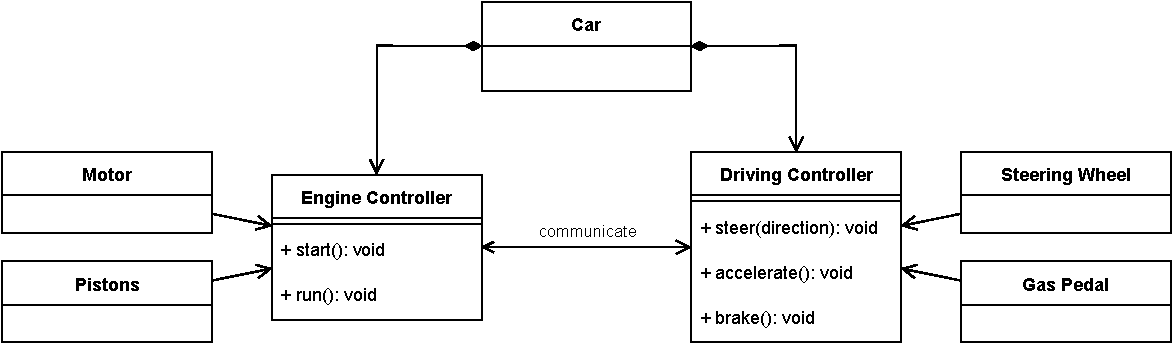
\includegraphics[width=\textwidth]{swt_h07_car.pdf}
            \end{center}
        \end{solution}
    \end{parts}
\end{questions}
\end{document}